\chapter{EXISTING TOOLS}
\label{existingVisualizationsChapter}
\section{Current Visualizations}
A number of visualization tools exist for exploration of food security, trade and climate change. Climate change models and future food insecurity indices are visualized on the \textit{Food Insecurity and Climate Change} website (figure \ref{metOffice}), hosted by the Met Office and World Food Programme (www.metoffice.gov.uk/food-insecurity-index). The website allows exploration of different scenarios of adaptation to climate change and greenhouse gas emissions. The visualization presents a long range (2050s and 2080s) forecast of the potential for food insecurity based on these factors.\par
\begin{figure}[htb]
	\center{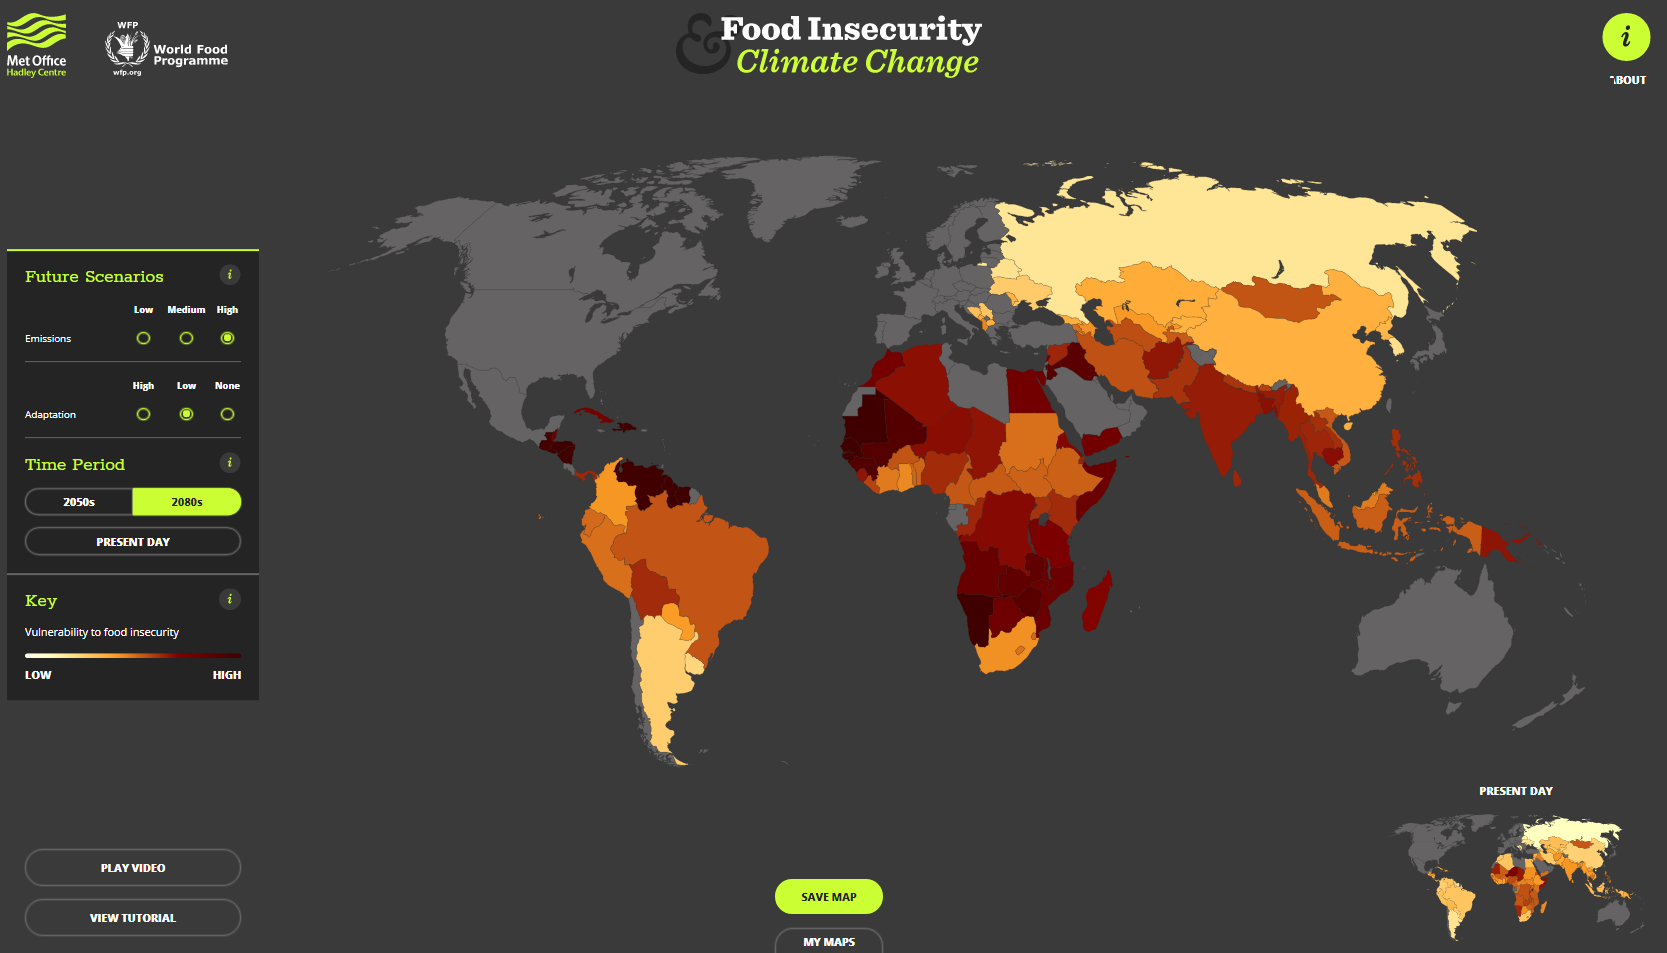
\includegraphics[width=\textwidth]{figures/metOffice.png}}
	\caption{Met Office Food Insecurity \& Climate Change website}
	\label{metOffice}
\end{figure}
Trade data can be visualized directly on the FAOSTAT website as seen in figure \ref{faostatViz} (www.fao.org/faostat/en/\#data/TM/visualize). This data visualization takes one country and displays the import or export trade links of a single trade good for that country. The visualization is done as a geographic choropleth representing the quantity or value of the imported or export good to another country. The visualization is limited as it only displays a single country's contribution and doesn't take into consideration the network as a whole.\par
\begin{figure}[htb]
	\center{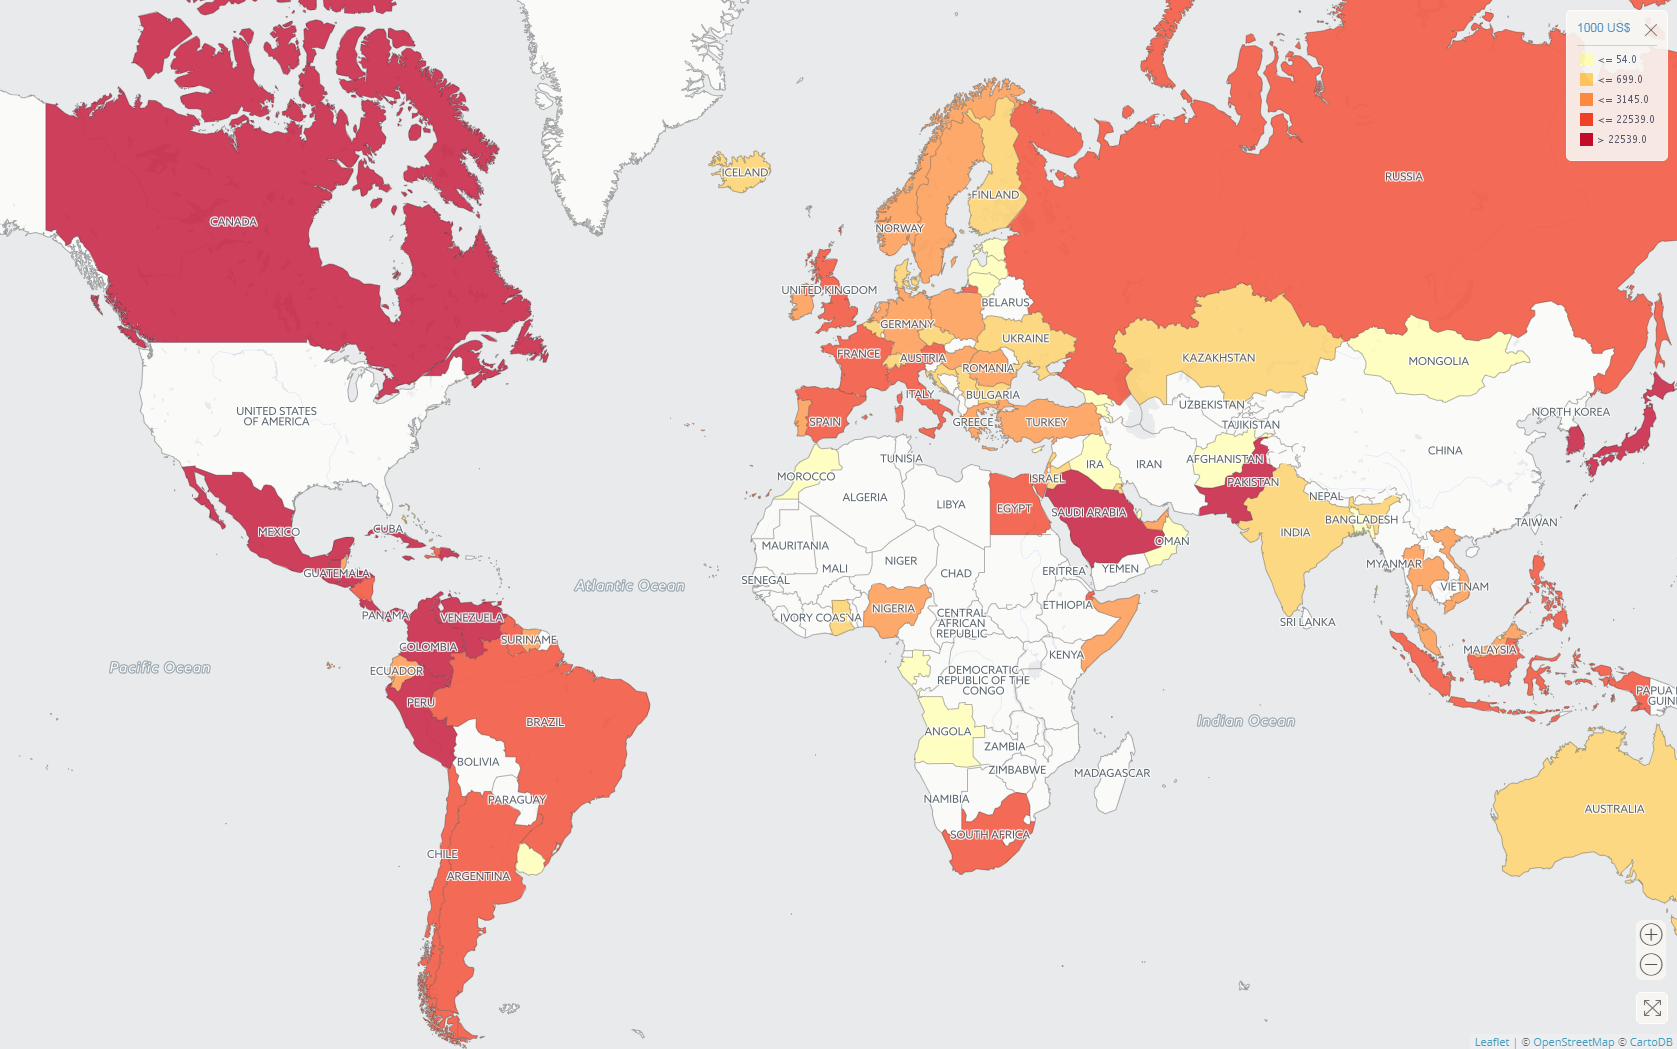
\includegraphics[width=\textwidth]{figures/faostatViz.png}}
	\caption{FAOSTAT Data Visualization tool}
	\label{faostatViz}
\end{figure}
\section{Enhancement Over the Existing Visualizations}
An emphasis of this visual analytics system is the consideration of the global trade network in its entirety. Neither of the reviewed visualizations take into consideration the topology of the food trade network. The FAOSTAT visualization represents only a single point in the food trade network. This does not allow for a direct interpretation of cascading effects. My tool visualizes the entire global trade network and allows for important network interpretations such as path length and network disconnections based on node and edge removal \citep{purchase1997aesthetic}. The visualization offered by the Met Office shows an index of food insecurity at a global scale. The focus is on overall vulnerability to food insecurity and does not visualize direct responses to climate events. The interaction and simulated climate events allow for the exploration of second order effects of climate events by direct visualization of the affected trade links in the network graph.\par
